\documentclass{article}

\usepackage{fancyhdr} % Required for custom headers
\usepackage{lastpage} % Required to determine the last page for the footer
\usepackage{extramarks} % Required for headers and footers
\usepackage{graphicx} % Required to insert images
\usepackage{lipsum} % Used for inserting dummy 'Lorem ipsum' text into the template
\usepackage{ctable}

% Margins
\topmargin=-0.45in
\evensidemargin=0in
\oddsidemargin=0in
\textwidth=6.5in
\textheight=9.0in
\headsep=0.25in 

\linespread{1.1} % Line spacing

% Set up the header and footer
\pagestyle{fancy}
\chead{\hmwkTitle} % Top center header
\renewcommand\headrulewidth{0.4pt} % Size of the header rule
\renewcommand\footrulewidth{0.4pt} % Size of the footer rule

\setlength\parindent{0pt} % Removes all indentation from paragraphs

% Header and footer for when a page split occurs within a problem environment
\newcommand{\enterProblemHeader}[1]{
\nobreak\extramarks{#1}{#1 continued on next page\ldots}\nobreak
\nobreak\extramarks{#1 (continued)}{#1 continued on next page\ldots}\nobreak
}

% Header and footer for when a page split occurs between problem environments
\newcommand{\exitProblemHeader}[1]{
\nobreak\extramarks{#1 (continued)}{#1 continued on next page\ldots}\nobreak
\nobreak\extramarks{#1}{}\nobreak
}

\setcounter{secnumdepth}{0} % Removes default section numbers
\newcounter{homeworkProblemCounter} % Creates a counter to keep track of the number of problems

\newcommand{\homeworkProblemName}{}
\newenvironment{homeworkProblem}[1][Question \arabic{homeworkProblemCounter}]{ % Makes a new environment called homeworkProblem which takes 1 argument (custom name) but the default is "Problem #"
\stepcounter{homeworkProblemCounter} % Increase counter for number of problems
\renewcommand{\homeworkProblemName}{#1} % Assign \homeworkProblemName the name of the problem
\section{\homeworkProblemName} % Make a section in the document with the custom problem count
\enterProblemHeader{\homeworkProblemName} % Header and footer within the environment
}{
\exitProblemHeader{\homeworkProblemName} % Header and footer after the environment
}

\newcommand{\problemAnswer}[1]{ % Defines the problem answer command with the content as the only argument
\noindent\framebox[\columnwidth][c]{\begin{minipage}{0.98\columnwidth}#1\end{minipage}} % Makes the box around the problem answer and puts the content inside
}

\newcommand{\homeworkSectionName}{}
\newenvironment{homeworkSection}[1]{ % New environment for sections within homework problems, takes 1 argument - the name of the section
\renewcommand{\homeworkSectionName}{#1} % Assign \homeworkSectionName to the name of the section from the environment argument
\subsection{\homeworkSectionName} % Make a subsection with the custom name of the subsection
\enterProblemHeader{\homeworkProblemName\ [\homeworkSectionName]} % Header and footer within the environment
}{
\enterProblemHeader{\homeworkProblemName} % Header and footer after the environment
}
   
%----------------------------------------------------------------------------------------
%       NAME AND CLASS SECTION
%----------------------------------------------------------------------------------------

\newcommand{\hmwkTitle}{Assignment\ 2\ report} % Assignment title
\newcommand{\hmwkDueDate}{Thursday,\ October\ 16,\ 2014} % Due date
\newcommand{\hmwkClass}{CS\ 5011}
\newcommand{\hmwkAuthorName}{Sure Manoj Kumar} % Your name

%----------------------------------------------------------------------------------------
%       TITLE PAGE
%----------------------------------------------------------------------------------------

\title{
\textmd{\textbf{\hmwkClass:\ \hmwkTitle}}\\
\normalsize\vspace{0.1in}\small{Due\ on\ \hmwkDueDate}\\
}

\author{\textbf{\hmwkAuthorName}}
\date{CS12B028} % Insert date here if you want it to appear below your name

%----------------------------------------------------------------------------------------

\begin{document}

\maketitle

\begin{homeworkProblem}[Question \arabic{homeworkProblemCounter}.]
The parameters are chosen based on the accuracy scores.\\
{\bf Linear} : 61.43\% accuracy\\\\
{\bf polynomial:}  \\
maximum accuracy - 68.58\% for degree=2 and gamma=2.\\\\
{\bf guassian(rbf):} \\
maximum accuracy - 69.68\% for gamma = 2 and C = 4 .\\\\
{\bf sigmoid:}\\
maximum accuracy - 54.37\% for gamma=1 and coef0=0 .\\\\
\end{homeworkProblem}

\begin{homeworkProblem}[Question \arabic{homeworkProblemCounter}.]
For the original back-propagation algorithm,the performance measures are:\\
parameters used $ \gamma_r = 0.01 $ and iterations=200.\\
Accuracy = 0.6125\\
Precision for coast = 1.0\\
Precision for forest = 0.90\\
Precision for insidecity = 0.54\\
Precision for mountain = 0.58\\
Recall for coast = 0.05\\
Recall for forest = 0.5\\
Recall for insidecity= 1.0\\
Recall for mountain = 0.9\\
F\_measure for coast = 0.095\\
F\_measure for forest = 0.64\\
F\_measure for insidecity = 0.7017\\
F\_measure for mountain = 0.7058\\
Updated rules for the new error function :
$$ \beta_{km}^{(r+1)} = \beta_{km}^{(r)} - \gamma_r (\sum_{i=1}^{N} (\frac{\partial R}{\partial \beta_{km}^{(r)}})+2 \gamma \beta_{km}^{(r)} ) $$
$$ \alpha_{ml}^{(r+1)} = \alpha_{ml}^{(r)} - \gamma_r( \sum_{i=1}^{N} (\frac{\partial R}{\partial \alpha_{ml}^{(r)}})+2 \gamma \alpha_{ml}^{(r)} ) $$
parameters used $ \gamma_r = 0.01 $ and iterations=100 and $ \gamma = 0.01 $.\\
Accuracy = 0.6875\\
Precision for coast = 0.6\\
Precision for forest = 0.73\\
Precision for insidecity = 0.75\\
Precision for mountain = 0.625\\
Recall for coast = 0.3\\
Recall for forest = 0.95\\
Recall for insidecity= 0.75\\
Recall for mountain = 0.75\\
F\_measure for coast = 0.4\\
F\_measure for forest = 0.82\\
F\_measure for insidecity = 0.75\\
F\_measure for mountain = 0.68\\\\
parameters used $ \gamma_r = 0.01 $ and iterations=100 and $ \gamma = 0.1 $.\\
Accuracy = 0.6625\\
Precision for coast = 0.63\\
Precision for forest = 0.65\\
Precision for insidecity = 0.66\\
Precision for mountain = 0.68\\
Recall for coast = 0.35\\
Recall for forest = 0.95\\
Recall for insidecity= 0.6\\
Recall for mountain = 0.75\\
F\_measure for coast = 0.45\\
F\_measure for forest = 0.77\\
F\_measure for insidecity = 0.63\\
F\_measure for mountain = 0.71\\\\
parameters used $ \gamma_r = 0.01 $ and iterations=100 and $ \gamma = 1 $.\\
Accuracy = 0.5625\\
Precision for coast = 0.55\\
Precision for forest = 0.62\\
Precision for insidecity = 0.47\\
Precision for mountain = 0.57\\
Recall for coast = 0.25\\
Recall for forest = 0.9\\
Recall for insidecity= 0.55\\
Recall for mountain = 0.55\\
F\_measure for coast = 0.34\\
F\_measure for forest = 0.73\\
F\_measure for insidecity = 0.51\\
F\_measure for mountain = 0.56\\\\
parameters used $ \gamma_r = 0.01 $ and iterations=50 and $ \gamma = 10 $.\\
Accuracy = 0.5375\\
Precision for coast = 0.41\\
Precision for forest = 0.62\\
Precision for insidecity = 0.48\\
Precision for mountain = 0.57\\
Recall for coast = 0.25\\
Recall for forest = 0.75\\
Recall for insidecity= 0.6\\
Recall for mountain = 0.55\\
F\_measure for coast = 0.31\\
F\_measure for forest = 0.68\\
F\_measure for insidecity = 0.53\\
F\_measure for mountain = 0.56\\\\
parameters used $ \gamma_r = 0.001 $ and iterations=25 and $ \gamma = 100 $.\\
Accuracy = 0.3\\
Precision for coast = 0.21\\
Precision for forest = 0\\
Precision for insidecity = 0.31\\
Precision for mountain = 0.33\\
Recall for coast = 0.25\\
Recall for forest = 0\\
Recall for insidecity= 0.20\\
Recall for mountain = 0.30\\
F\_measure for coast =0.22 \\
F\_measure for forest = -\\
F\_measure for insidecity = 0.30\\
F\_measure for mountain =0.31 \\\\
The new error function is similar to adding ridge in ridge regression.The advantage of this error function is numerical values of weights will be low as compared to previous weights which were derived from original back propagation algorithm.This is because,we have added weights also in the error term ,which makes the numerical values of weights to be low.The more the value of $\gamma$ the less the values of weights.and as $\gamma$ increases the accuracy/performance decreases.As the value of the gamma increases,the function will try to minimise the weights rather than error caused due to mis-classification which makes the accuracy to drop as the value of gamma increases.
\end{homeworkProblem}

\begin{homeworkProblem}[Question \arabic{homeworkProblemCounter}.]
For L2 logistic regression, the performance measures are\\
Accuracy - 0.95\\
Precision for forest class - 1.0\\
Precision for mountain class  - 0.909090909091\\
Recall for forest class - 0.9\\
Recall for mountain class - 1.0\\
F-measure for forest class - 0.947368421053\\
F-measure for mountain class - 0.952380952381\\\\


For L1 logistic regression using Boyd's code ,the performance measures are \(for\; \lambda = 0.01\)\\
Accuracy - 0.975\\
Precision for forest class - 1.0\\
Precision for mountain class - 0.952380952381\\
Recall for forest class - 0.95\\
Recall for mountain class - 1.0\\
F-measure for forest class - 0.974358974359\\
F-measure for mountain class - 0.975609756098 \\\\
\end{homeworkProblem}


\begin{homeworkProblem}[Question \arabic{homeworkProblemCounter}.]

\begin{figure}[h!]
\centering
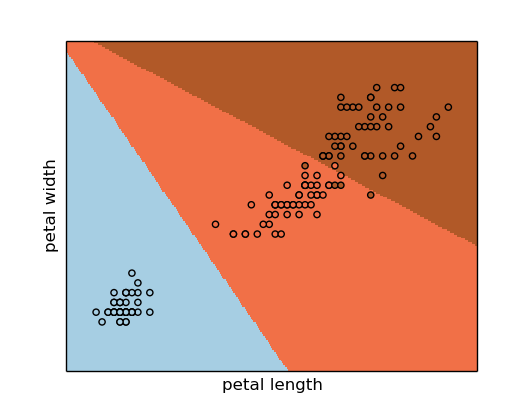
\includegraphics[width=0.5\textwidth]{figure_1.png}
\caption{LDA}
\end{figure}
\begin{figure}[h!]
\centering
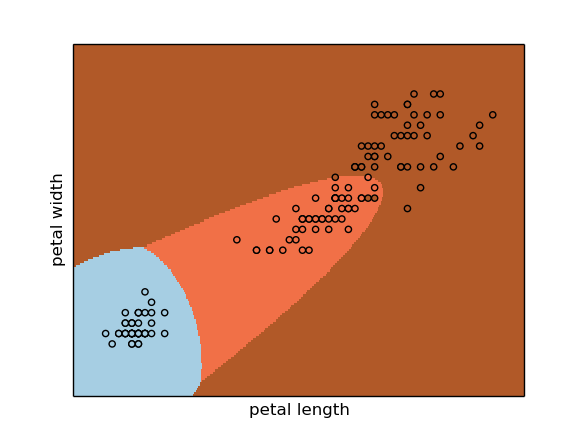
\includegraphics[width=0.5\textwidth]{figure_2.png}
\caption{QDA}
\end{figure}
\begin{figure}[h!]
\centering
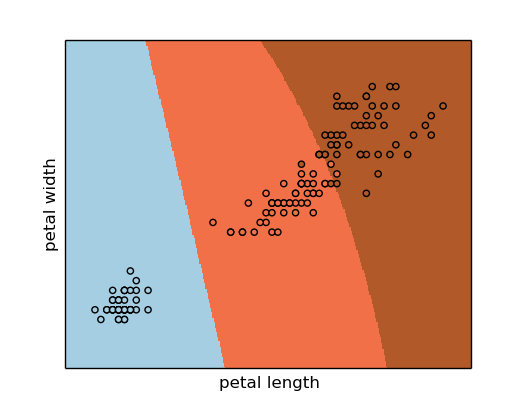
\includegraphics[width=0.5\textwidth]{figure_3.png}
\caption{RDA with regparam as 0.3}
\end{figure}
\end{homeworkProblem}
\end{document}